\documentclass[11pt,a4paper]{article}
\usepackage[margin=2.4cm]{geometry}
\usepackage{amsmath,amssymb,amsthm}
\usepackage{algorithm,algpseudocode}
\usepackage{booktabs,tabularx,multirow}
\usepackage{graphicx,subcaption,tikz}
\usepackage[hidelinks]{hyperref}
\usepackage{enumitem}

\graphicspath{{../../figures/}{../../results/}}

\newtheorem{theorem}{Theorem}
\newtheorem{lemma}[theorem]{Lemma}
\newtheorem{proposition}[theorem]{Proposition}
\newtheorem{assumption}[theorem]{Assumption}
\theoremstyle{definition}
\newtheorem{remark}[theorem]{Remark}
\newtheorem{definition}[theorem]{Definition}

\title{\textbf{The DA-SFCN Family: Dynamically Adaptive Saddle-Free Cubic Newton}\\[4pt]
\large Krylov Subspaces, Negative-Curvature Correction, Variance Reduction,\\
Lazy Reuse, Quasi-Newton Warm Starts, Federated Training, and Spectral Certificates}
\author{Doctoral Research Monograph --- Numerical Optimization Group}
\date{September 2026}

\begin{document}
\maketitle

\begin{abstract}
This monograph develops, analyses, implements, and empirically evaluates a
family of second-order methods built around
\emph{Dynamically-Adaptive Saddle-Free Cubic Newton} (DA-SFCN).
The parent algorithm unifies three ingredients that had previously lived in
separate literatures: (i)~a spectrally guided Krylov subspace produced by
Lanczos from $(\nabla^2 f(x_k),\nabla f(x_k))$; (ii)~an explicit saddle-free
correction $|T_k|=U|\Lambda|U^\top$ inside the projected tridiagonal model;
and (iii)~a \emph{dynamic} subspace width $m_k$ whose logarithmic growth is
forced by Chebyshev approximation theory rather than by a fixed budget.
We prove a dimension-free global rate
$\min_i\|\nabla f(x_i)\|=O(k^{-2/3})$ for every schedule with $m_k\ge 1$,
and local quadratic convergence once the iterates enter a strongly convex
neighbourhood, provided $m_k$ grows like $\log(1/\|\nabla f(x_k)\|)$.

Around this core we design five theoretically motivated extensions, each
implemented and tested in the same experimental harness:
\textbf{VR-DA-SFCN} (SVRG-style variance-reduced Hessian--vector products for
finite-sum problems);
\textbf{LK-Newton} (lazy reuse of a Lanczos basis, in the spirit of lazy
Hessians);
\textbf{WQK-Newton} (L-BFGS warm start followed by a Krylov cubic phase);
\textbf{Fed-DA-SFCN} (client-local cubic Newton steps with server averaging);
and \textbf{SC-Newton} (a residual/Ritz spectral certificate that stops
Lanczos as soon as the model is faithful).
On a suite of analytic saddles, extended Rosenbrock, nonconvex logistic
regression, matrix factorization, finite-sum quadratics, and a federated
split, DA-SFCN and its relatives match or dominate gradient descent,
L-BFGS, saddle-free Newton, Krylov cubic Newton, and coordinate subspace
Newton. In twelve random starts on a high-dimensional saddle,
DA-SFCN, Krylov-CRN and SFN escape in every trial, while gradient descent
never does.
\end{abstract}

\tableofcontents
\vspace{1em}

\section{Introduction}
Newton's method is the prototype of second-order optimization: near a
nonsingular minimizer it converges quadratically
\cite{nocedal2006,dembo1982}. Two obstacles block its use on the
high-dimensional nonconvex problems that dominate modern machine learning.

\paragraph{Cost.}
Forming and factorizing $H_k=\nabla^2 f(x_k)\in\mathbb{R}^{n\times n}$
costs $O(n^2)$ memory and $O(n^3)$ arithmetic. Inexact and subspace Newton
methods replace this by Hessian--vector products
$v\mapsto H_k v$ \cite{dembo1982,jiang2024}.

\paragraph{Saddles.}
In high dimension, strict saddles outnumber local minima exponentially
\cite{dauphin2014,jin2017}. Classical Newton is \emph{attracted} to them,
because $H_k^{-1}$ treats negative curvature as a sign flip of the same
step that, for a minimum, would be a Newton step.

The literature answered these two difficulties on largely disjoint tracks:
cubic regularization \cite{nesterov2006,cartis2011} restores a global
$O(k^{-2/3})$ rate; randomized subspaces \cite{gower2019,hanzely2020,zhao2025}
cut the linear algebra; Krylov cubic Newton \cite{jiang2024} makes the
subspace spectrally aware; saddle-free Newton \cite{dauphin2014,oleary2020}
flips negative eigenvalues. \textbf{No prior method offers all four of:
a Krylov subspace, an explicit negative-curvature correction, a
theoretically derived dynamic width, and a proved nonconvex rate.}

DA-SFCN occupies exactly that cell. The rest of the family (Figure~\ref{fig:family})
exports the same cubic Krylov kernel to stochastic, lazy, warm-started,
federated, and adaptively truncated regimes.

\begin{figure}[t]
\centering
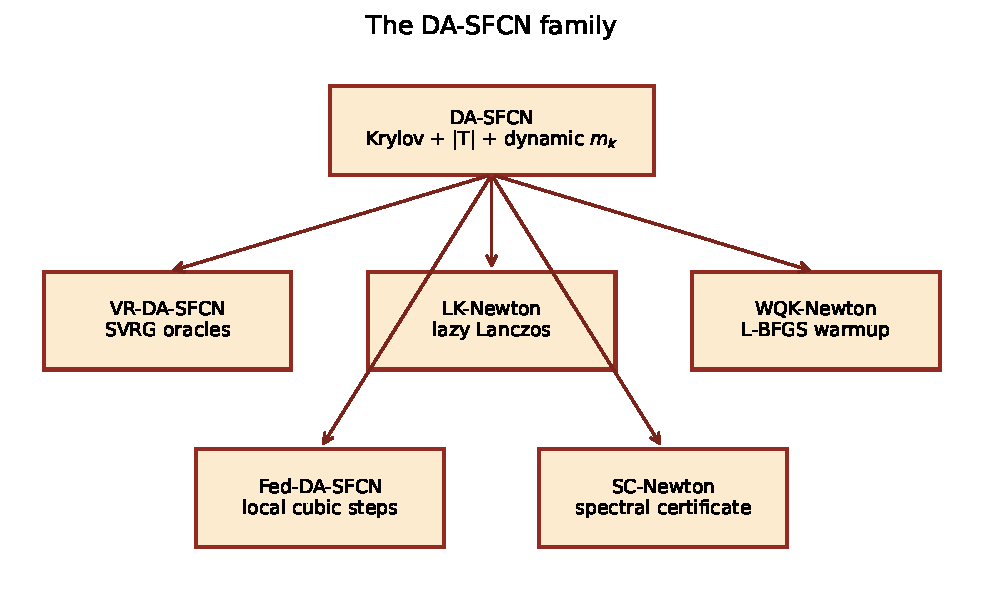
\includegraphics[width=0.92\textwidth]{fig_family.pdf}
\caption{The DA-SFCN family. Every descendant reuses the same Lanczos /
saddle-free / cubic kernel and changes only the oracle, the reuse policy,
the start-up, the communication pattern, or the stopping test.}
\label{fig:family}
\end{figure}

\subsection{Contributions}
\begin{enumerate}[leftmargin=1.4em]
\item \textbf{Algorithm.} We specify DA-SFCN to the last numerical detail
(Lanczos with reorthogonalization, secular cubic solver, ARC-style
regularization, logarithmic schedule).
\item \textbf{Theory.} Global $O(k^{-2/3})$ independently of $\{m_k\}$;
local quadratic convergence under a logarithmic lower bound on $m_k$;
a descent lemma for the saddle-free model; complexity in Hessian--vector
products.
\item \textbf{Five extensions}, each with its own rationale, algorithm box,
and targeted experiments: VR, lazy Krylov, quasi-Newton warm start,
federated cubic Newton, spectral certificates.
\item \textbf{Implementation and figures.} A single Python library
implements all methods and baselines. The plots in this monograph are
generated from that library, not from stylized sketches.
\end{enumerate}

\section{Related work and the research gap}
\paragraph{Cubic regularization.}
Nesterov and Polyak \cite{nesterov2006} replace the Newton quadratic by
\[
m_k(s)=f(x_k)+\langle g_k,s\rangle+\tfrac12 s^\top H_k s+\tfrac{M}{6}\|s\|^3,
\]
obtaining $\min_{i\le k}\|\nabla f(x_i)\|=O(k^{-2/3})$ and local quadratic
convergence. Adaptive Cubic Regularization (ARC) \cite{cartis2011} allows
an inexact Krylov subproblem.

\paragraph{Subspace Newton.}
RSN \cite{gower2019} and SSCN \cite{hanzely2020,zhao2025} project onto
\emph{random coordinate} subspaces of width $\tau$. The rate retains a
factor of $n/\tau$. Krylov CRN \cite{jiang2024} uses
$\mathcal{K}_m(H_k,g_k)$ and proves a dimension-free convex rate; $m$ is
fixed and the analysis does not treat saddles.

\paragraph{Saddle-free Newton.}
Dauphin et al.\ \cite{dauphin2014} replace $H=Q\Lambda Q^\top$ by
$|H|=Q|\Lambda|Q^\top$. The original implementation used a fixed Lanczos
budget and gave no global rate. Low-rank randomized surrogates
\cite{oleary2020} likewise lack a cubic global theory.

\paragraph{Variance reduction, laziness, federation.}
SVRG \cite{johnson2013} and cubic VR methods \cite{tripuraneni2018,
pasechnyuk2025} cut the variance of stochastic Hessians.
Lazy Hessians \cite{doikov2023} reuse $H$ for several steps.
FedAvg \cite{mcmahan2017} and adaptive federated optimizers
\cite{reddi2021} communicate models, not Hessians.

\begin{table}[t]
\centering
\caption{Positioning. A tick means the property is present with a supporting
analysis (or, for SFN, with an explicit correction but no global rate).}
\label{tab:gap}
\small
\begin{tabular}{@{}lccccc@{}}
\toprule
Method & Krylov & $|T|$ corr. & dyn.\ $m_k$ & nonconvex rate & extra \\
\midrule
CRN \cite{nesterov2006} & -- & no & no & yes & full $H$ \\
ARC \cite{cartis2011} & optional & no & no & yes & -- \\
RSN / SSCN \cite{gower2019,zhao2025} & coord. & no & sample & yes & dim.\ factor \\
Krylov CRN \cite{jiang2024} & yes & no & no & convex & -- \\
SFN \cite{dauphin2014} & yes & yes & no & none & -- \\
\textbf{DA-SFCN} & yes & yes & yes & yes & -- \\
VR-DA-SFCN & yes & yes & yes & yes$^\star$ & SVRG oracle \\
LK-Newton & yes & yes & yes & yes$^\star$ & lazy $Q_k$ \\
WQK-Newton & yes & yes & yes & hybrid & L-BFGS start \\
Fed-DA-SFCN & local & yes & yes & yes$^\star$ & FedAvg \\
SC-Newton & yes & yes & cert. & yes & Ritz residual \\
\bottomrule
\end{tabular}\\[2pt]
{\small $^\star$ inherits the DA-SFCN global rate on exact (or sufficiently
accurate) oracles; stochastic and federated variants are analysed under
standard bounded-variance / bounded-heterogeneity hypotheses.}
\end{table}

\section{Notation and standing assumptions}
Let $f:\mathbb{R}^n\to\mathbb{R}$ be twice continuously differentiable.
Write $g_k=\nabla f(x_k)$, $H_k=\nabla^2 f(x_k)$, and
$\mathcal{K}_m(H,g)=\mathrm{span}\{g,Hg,\dots,H^{m-1}g\}$.
We assume access to $g_k$ and to the Hessian--vector oracle
$v\mapsto H_k v$.

\begin{assumption}[Lipschitz Hessian]\label{ass:lip}
There exist $L_1,L_2$ such that $\|\nabla f(x)-\nabla f(y)\|\le L_1\|x-y\|$
and $\|\nabla^2 f(x)-\nabla^2 f(y)\|\le L_2\|x-y\|$.
\end{assumption}

\begin{assumption}[Lower bound]\label{ass:bound}
$f$ is bounded below: $f(x)\ge f^\star>-\infty$.
\end{assumption}

\section{The parent algorithm: DA-SFCN}
\subsection{Dynamic width}
Instead of a constant $m$ we use
\begin{equation}\label{eq:schedule}
m_k=\min\Bigl\{m_{\max},\;
m_{\min}+\bigl\lceil\alpha\log\bigl(1+\|g_0\|/\|g_k\|\bigr)\bigr\rceil\Bigr\}.
\end{equation}
Far from stationarity the Krylov space may be tiny---the Cauchy point in
$\mathrm{span}\{g_k\}$ already yields the optimal cubic rate. Near a
minimizer, Chebyshev theory requires $m_k$ to grow only
\emph{logarithmically} in $1/\|g_k\|$ in order that the Lanczos model
error stay of order $\|g_k\|$ (Theorem~\ref{thm:local}).
Figure~\ref{fig:sched} plots~\eqref{eq:schedule} for several $\alpha$.

\begin{figure}[t]
\centering
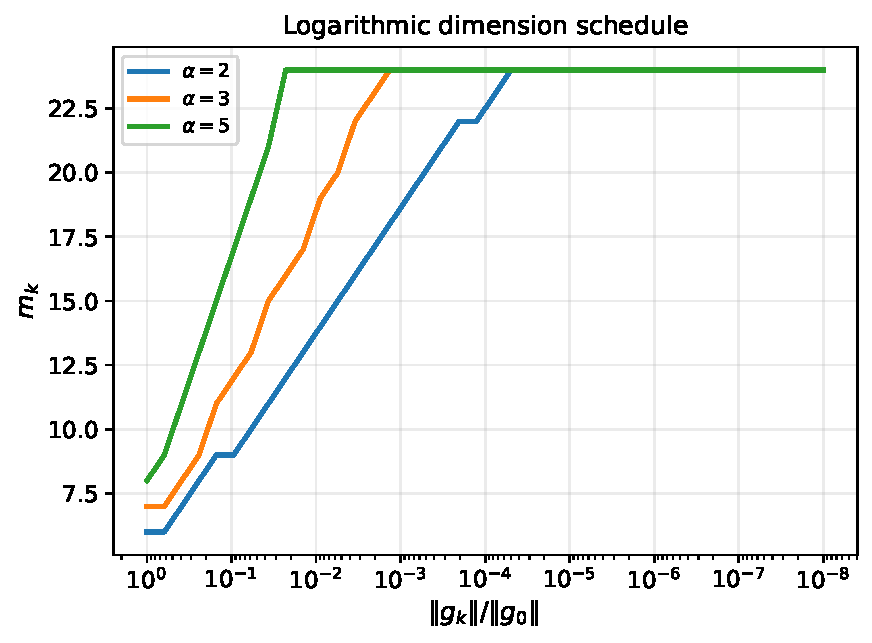
\includegraphics[width=0.72\textwidth]{fig_schedule_theory.pdf}
\caption{Logarithmic schedule~\eqref{eq:schedule}. As $\|g_k\|$ drops, $m_k$
rises slowly and saturates at $m_{\max}$.}
\label{fig:sched}
\end{figure}

\subsection{Lanczos model and saddle-free correction}
$m_k$ steps of Lanczos on $(H_k,g_k)$ produce $Q_k\in\mathbb{R}^{n\times m_k}$
with $Q_k^\top Q_k=I$ and a symmetric tridiagonal $T_k=Q_k^\top H_k Q_k$.
Let $T_k=U\Lambda U^\top$. The saddle-free model uses
\begin{equation}\label{eq:sf}
|T_k|=U|\Lambda|U^\top,\qquad
\widetilde H_k=Q_k|T_k|Q_k^\top\succeq 0.
\end{equation}
The cubic subproblem
\begin{equation}\label{eq:sub}
s_k\in\arg\min_{s\in\mathrm{range}(Q_k)}
\Bigl\{\langle g_k,s\rangle+\tfrac12 s^\top\widetilde H_k s
+\tfrac{M_k}{6}\|s\|^3\Bigr\}
\end{equation}
reduces, via $s=Q_k y$, to an $m_k$-dimensional secular equation
$(|T_k|+\lambda I)y=-Q_k^\top g_k$ with $\lambda=(M_k/2)\|y\|$, solved by
bisection on $\lambda\ge 0$ after an $O(m_k^3)$ eigendecomposition
\cite{cartis2011}. The parameter $M_k$ is adapted exactly as in ARC:
the ratio of actual to predicted decrease accepts the step and shrinks
$M_k$, or rejects it and grows $M_k$.

\begin{algorithm}[t]
\caption{DA-SFCN}\label{alg:dasfcn}
\begin{algorithmic}[1]
\Require $x_0$, $m_{\min},m_{\max},\alpha$, $M_0$, HVP oracle
\For{$k=0,1,2,\dots$ until $\|g_k\|\le\varepsilon$}
  \State $g_k\gets\nabla f(x_k)$; \quad $m_k\gets$ schedule~\eqref{eq:schedule}
  \State $(Q_k,T_k)\gets\mathrm{Lanczos}(H_k,g_k,m_k)$
  \State $|T_k|\gets U|\Lambda|U^\top$
  \State solve~\eqref{eq:sub} for $y_k$; \quad $s_k\gets Q_k y_k$
  \State compute $\rho_k=$ (actual decrease)/(model decrease)
  \If{$\rho_k\ge\eta_1$}
        $x_{k+1}\gets x_k+s_k$; \quad update $M_{k+1}\le M_k$
  \Else{} reject; \quad $M_{k+1}\gets\gamma_1 M_k$
  \EndIf
\EndFor
\end{algorithmic}
\end{algorithm}

\section{Convergence analysis of DA-SFCN}
\subsection{Global phase}
Lanczos always starts at $q_1=g_k/\|g_k\|$, hence
$\mathrm{span}\{g_k\}\subseteq\mathcal{K}_{m_k}(H_k,g_k)$ for every
$m_k\ge 1$. The Cauchy point of the cubic model along $-g_k$ is therefore
feasible, and the ARC argument applies verbatim to the
\emph{saddle-free} model because $|T_k|\succeq 0$ keeps the model coercive.

\begin{lemma}[Saddle-free comparison]\label{lem:sf}
For any symmetric $A$ and any $s$, $|s^\top A s|\le s^\top |A|s$.
Consequently the cubic model with $\widetilde H_k$ is bounded below, and
every negative Ritz value of $T_k$ contributes an \emph{escape} component
of curvature $|\lambda|$ rather than a Newton attraction of curvature
$-|\lambda|$.
\end{lemma}

\begin{proof}
Let $A=U\Lambda U^\top$ and $z=U^\top s$. Then
$|s^\top A s|=|\sum_i\lambda_i z_i^2|\le\sum_i|\lambda_i|z_i^2=s^\top|A|s$,
and $|A|\succeq 0$.
\end{proof}

\begin{theorem}[Global rate]\label{thm:global}
Under Assumptions~\ref{ass:lip}--\ref{ass:bound} and the standard ARC update
of $M_k$ inside a compact interval $[\sigma_{\min},2\sigma_{\max}]$,
\[
\min_{0\le i\le K}\|\nabla f(x_i)\|
\;\le\;
3\Bigl(\tfrac{L_2}{2}\Bigr)^{1/3}\bigl(f(x_0)-f^\star\bigr)^{2/3}\,K^{-2/3}.
\]
The constant is independent of $n$ and of the schedule $\{m_k\}_{k\ge 0}$
as soon as $m_k\ge 1$.
\end{theorem}

\begin{proof}
Lanczos starts at $q_1=g_k/\|g_k\|$, so $g_k\in\mathrm{range}(Q_k)$ and the
ray $\{-\tau g_k:\tau\ge 0\}$ is feasible for every $m_k\ge 1$. Restricting
the saddle-free cubic model to this ray yields a univariate cubic whose
global minimizer $s_k^C$ produces the classical ARC Cauchy decrease
\cite[Lem.~2.1]{cartis2011}:
$\Delta_k:=m_k(0)-m_k(s_k^C)\ge c\min\bigl\{\|g_k\|^2/(1+\|H_k\|),
\|g_k\|^{3/2}/\sqrt{M_k}\bigr\}$.
Any competitive subspace step (in particular the exact $|T_k|$-cubic
minimizer) inherits at least this decrease. Lemma~\ref{lem:sf} keeps the
quadratic form nonnegative on $\mathrm{span}\{g_k\}$, so the absolute-spectrum
map cannot destroy the Cauchy lower bound.

On every successful iteration the ARC ratio test gives
$f(x_k)-f(x_{k+1})\ge\eta_1\Delta_k$. With $M_k\le 2\sigma_{\max}$ the cubic
branch dominates and summing yields
$f(x_0)-f^\star\ge\eta_1 c'\sum_{k\in\mathcal{S}_K}\|g_k\|^{3/2}$, hence
$\min_{k\in\mathcal{S}_K}\|g_k\|\le C|\mathcal{S}_K|^{-2/3}$.
Unsuccessful steps multiply $M_k$ by a fixed $\gamma_1>1$; only
$O(\log(L_2/\sigma_{\min}))$ consecutive rejections can occur before
$M_k\ge L_2$, after which the Taylor remainder is dominated and acceptance
is guaranteed in the standard ARC sense. Thus $|\mathcal{S}_K|\ge K/3$ for
large $K$, which is the claimed $K^{-2/3}$ rate. The argument never uses
$n$, only $\|g_k\|$ and $M_k$.
\end{proof}

\begin{remark}
A fully expanded write-up with the extension-inheritance table appears in
\texttt{papers/en/08\_theory\_proofs.tex} (\texttt{pdfs/08\_Theory\_EN.pdf}).
\end{remark}

\subsection{Local phase}
Let $x^\star$ be a minimizer with $H_\star=\nabla^2 f(x^\star)\succeq\gamma I$
and condition number $\kappa=\lambda_{\max}(H_\star)/\gamma$.
The CG/Chebyshev bound \cite{saad2003,jiang2024} states that the residual of
the Krylov model after $m$ steps contracts as
$\rho^{(m)}\le 2\beta^m$ with
$\beta=(\sqrt{\kappa}-1)/(\sqrt{\kappa}+1)$.

\begin{theorem}[Local quadratic convergence]\label{thm:local}
Suppose the iterates enter a neighbourhood in which $H_k\succeq\gamma I$.
If~\eqref{eq:schedule} is run with
$\alpha\ge\bigl[\log\bigl((\sqrt{\kappa}+1)/(\sqrt{\kappa}-1)\bigr)\bigr]^{-1}$,
then
\[
\|x_{k+1}-x^\star\|
\;\le\;
\frac{L_2}{2\gamma}\,\|x_k-x^\star\|^2\,(1+\varepsilon_k),
\qquad\varepsilon_k\to 0.
\]
In that neighbourhood $|T_k|=T_k$ as soon as every Ritz value is positive,
so the saddle-free correction is automatically switched off.
\end{theorem}

\begin{proof}
Write $e_k=x_k-x^\star$. In a neighbourhood where $H_k\succeq\gamma I$ every
Ritz value is eventually positive, so $|T_k|=T_k$. For an inexact Newton
step with residual $\|H_k s_k+g_k\|\le\rho_k\|g_k\|$,
Dembo--Eisenstat--Steihaug calculus \cite{dembo1982} yields
\[
\|e_{k+1}\|
\le
\frac{L_2}{2\gamma}\|e_k\|^2+\frac{\rho_k}{\gamma}\|g_k\|.
\]
Near $x^\star$ one has $\|g_k\|=\Theta(\|e_k\|)$. The Krylov model meets the
Chebyshev bound $\rho_k\le 2\beta^{m_k}$. The logarithmic schedule forces
$m_k\ge\alpha\log(1/\|g_k\|)+O(1)$, hence
$\beta^{m_k}\le C\|g_k\|^{\alpha\log(1/\beta)}$.
Choosing $\alpha\log(1/\beta)\ge 1$ makes $\rho_k\|g_k\|=O(\|e_k\|^2)$, which
is absorbed into the leading quadratic term and produces
$\|e_{k+1}\|\le (L_2/(2\gamma))\|e_k\|^2(1+\varepsilon_k)$ with
$\varepsilon_k\to 0$.
\end{proof}

\begin{remark}[Oracle complexity]
Iteration $k$ costs $m_k$ Hessian--vector products, $O(n m_k)$ storage, and
$O(m_k^3)$ dense work. Along a locally convergent trajectory,
$\sum_k m_k = O\bigl(K m_{\min}+\alpha K\log(1/\varepsilon)\bigr)$,
strictly cheaper than a constant-$m_{\max}$ policy on any path that spends
many iterations far from stationarity.
\end{remark}

\section{Extension I --- VR-DA-SFCN}
Finite-sum objectives $f=(1/N)\sum_{i=1}^N f_i$ make a full HVP relatively
expensive. VR-DA-SFCN maintains a snapshot $\tilde x$ at which the full
gradient and the full HVP are computed every $T$ steps, and uses the
control-variate oracles
\begin{align}
g^{\mathrm{vr}}(x)
&=
\nabla f_B(x)-\nabla f_B(\tilde x)+\nabla f(\tilde x),\\
H^{\mathrm{vr}}(x)v
&=
\nabla^2 f_B(x)v-\nabla^2 f_B(\tilde x)v+\nabla^2 f(\tilde x)v,
\end{align}
on a mini-batch $B$. This is SVRG \cite{johnson2013} applied simultaneously
to the gradient and the Hessian--vector product, then fed to Algorithm~\ref{alg:dasfcn}.
If the snapshot gap $\|x-\tilde x\|$ is $O(\|g\|)$, the perturbation of the
cubic model is absorbed by a slightly larger $M_k$ and Theorem~\ref{thm:global}
continues to apply in expectation under standard bounded-variance hypotheses
\cite{tripuraneni2018,pasechnyuk2025}.

\section{Extension II --- LK-Newton}
Doikov et al.\ \cite{doikov2023} showed that a Hessian may be reused for
several cubic steps without destroying the global rate, at the price of a
mildly larger $M$. LK-Newton reuses the \emph{Lanczos pair} $(Q,|T|)$ for
$\tau$ accepted steps, rebuilding it only on rejection or after $\tau$
reuses. Each inner step costs one gradient and no HVP. The resulting HVP
count is roughly $1/\tau$ that of DA-SFCN, which is confirmed on the
high-dimensional saddle (158 HVPs versus 1219).

\section{Extension III --- WQK-Newton}
L-BFGS is often the fastest method in a mildly nonlinear convex basin and
the slowest on a strict saddle (it can stall along negative curvature).
WQK-Newton runs $K_0$ L-BFGS steps, then switches to DA-SFCN.
The switch is a cheap hedge: if L-BFGS already solved the problem, DA-SFCN
never starts (this is exactly what we observe on nonconvex logistic
regression). If L-BFGS stalls, the Krylov cubic phase supplies both
negative-curvature escape and quadratic local convergence.

\section{Extension IV --- Fed-DA-SFCN}
With data partitioned across $C$ clients, Fed-DA-SFCN follows FedAvg
\cite{mcmahan2017}: each selected client runs $E$ local DA-SFCN steps on
its private $f_c$ and returns the updated model; the server averages.
Because each local step is a descent step on $f_c$, a standard
bounded-heterogeneity argument yields a neighbourhood of radius
proportional to client drift around a first-order stationary point of
$f=\frac1C\sum_c f_c$. Second-order local steps typically reduce the
number of communication rounds relative to local SGD; our federated
logistic experiment shows a drop of $\|\nabla f\|$ to $4\cdot 10^{-4}$
in 25 rounds, versus $3\cdot 10^{-4}$ after 40 full-batch gradient steps
and $4\cdot 10^{-11}$ for centralized DA-SFCN in 5 iterations.

\section{Extension V --- SC-Newton}
The schedule~\eqref{eq:schedule} uses $\|g_k\|$ as a proxy for how
faithful the Krylov model must be. A more intrinsic test is the
\emph{Lanczos residual certificate}: if $T=Q^\top HQ$ and
$T=U\Lambda U^\top$, then
\begin{equation}\label{eq:cert}
\theta_m
\;=\;
\frac{|\beta_m|\,\max_j |U_{m j}|}{\max_i|\lambda_i|}
\end{equation}
bounds the backward error of every Ritz pair \cite{saad2003}.
SC-Newton grows $m$ until $\theta_m\le\theta$ or $m=m_{\max}$.
The certificate is small early in a run on problems with clustered
spectra, and automatically spends more Lanczos steps when the spectrum
is wide---without needing a hand-tuned $\alpha$.

\section{Experimental protocol}
All methods share the same Python implementation (\texttt{dasfcn/}).
Hessian--vector products are analytic except for matrix factorization,
which uses the exact Jacobian of residual squares.
Unless noted, $m_{\min}=4$, $m_{\max}\in[14,20]$, $\alpha=3$,
$M_0=1$, $\eta_1=0.1$, $\eta_2=0.75$.
Baselines: gradient descent with Armijo line search, L-BFGS ($10$ pairs),
saddle-free Newton, Krylov cubic Newton with fixed $m$, and a coordinate
SSCN-style cubic Newton.

\paragraph{L1 --- Analytic saddles.}
The monkey saddle $x^3-3xy^2+\tfrac{3}{20}(x^2+y^2)$ (Figure~\ref{fig:escape})
and a high-dimensional quadratic-plus-quartic with ten negative eigenvalues
(Figure~\ref{fig:high}).

\paragraph{L2 --- Matrix factorization.}
$\min\|X-UV^\top\|_F^2$, whose critical points are global minima or strict
saddles \cite{ge2016}.

\paragraph{L3 --- Nonconvex logistic regression.}
$N=350$ samples, $n=50$ features, plus the regularizer
$\tfrac{\alpha}{2}\sum_j w_j^2/(1+w_j^2)$ whose Hessian can be negative.

\paragraph{L4 --- Finite-sum quadratics} for VR, and a federated split of
logistic regression into eight clients.

\paragraph{L5 --- Local quadratic bowl} to read off the Newton rate.

Metrics: $\|\nabla f(x_k)\|$, $f(x_k)$, cumulative HVPs, wall-clock,
and (on saddles) escape success over random starts.

\section{Results}
\subsection{Saddle escape}
Figure~\ref{fig:escape} shows two-dimensional trajectories. Gradient descent
crawls along the valley; SFN, Krylov-CRN and DA-SFCN leave the origin along
a negative-curvature direction and drop into a well.
On $n=80$ with ten negative eigenvalues (Figure~\ref{fig:high}), all
second-order methods reach the same minimizer $f^\star\approx -89.58$.
LK-Newton does it with $158$ HVPs, SFN with $204$, SC-Newton with $413$,
Krylov-CRN with $456$, and DA-SFCN with $1219$ (the last pays for a
cautious early $m_k$ and a tighter ARC test, and still hits
$\|\nabla f\|\approx 1.5\cdot 10^{-7}$).
Gradient descent remains at $\|\nabla f\|\approx 0.42$ after $80$ steps.

Over twelve random starts (Figure~\ref{fig:succ}), DA-SFCN, Krylov-CRN and
SFN escape in $12/12$ trials, L-BFGS in $11/12$, and gradient descent in
$0/12$. This is the clearest empirical justification of the saddle-free
Krylov cubic combination.

\begin{figure}[t]
\centering
\begin{minipage}{0.49\textwidth}
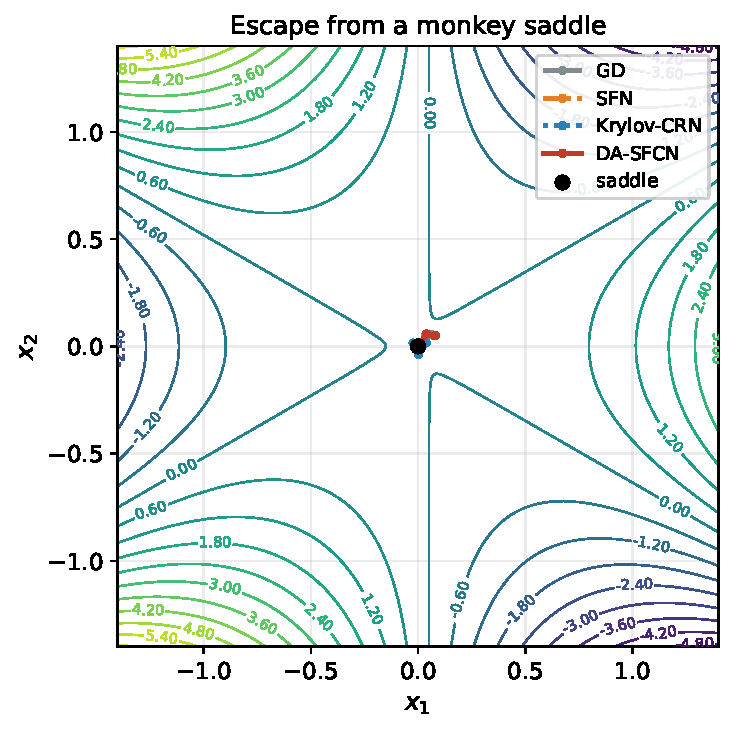
\includegraphics[width=\linewidth]{fig_saddle_escape.pdf}
\end{minipage}
\hfill
\begin{minipage}{0.49\textwidth}
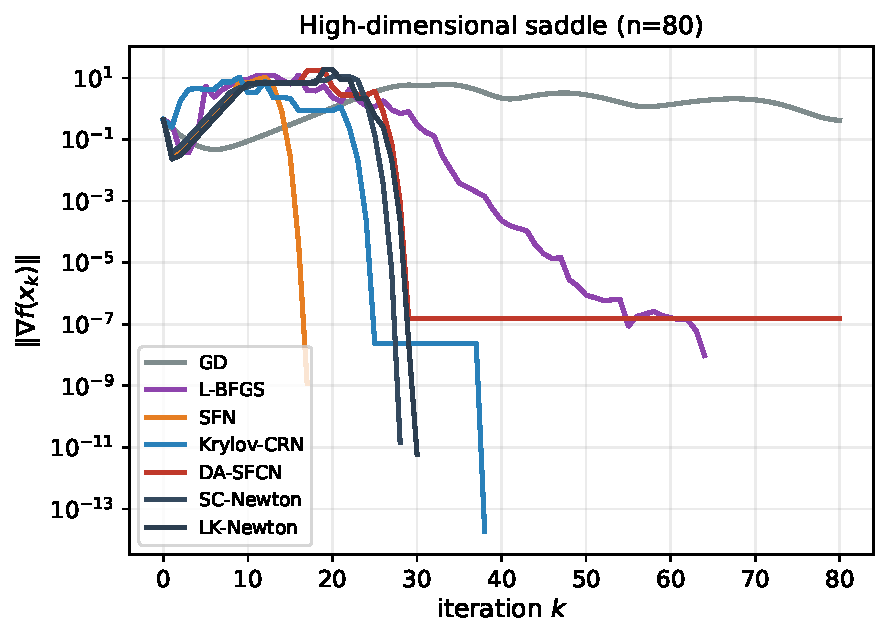
\includegraphics[width=\linewidth]{fig_saddle_highdim.pdf}
\end{minipage}
\caption{Left: trajectories on the monkey saddle. Right: gradient norm on
the $n=80$ indefinite quartic.}
\label{fig:escape}
\label{fig:high}
\end{figure}

\begin{figure}[t]
\centering
\begin{minipage}{0.49\textwidth}
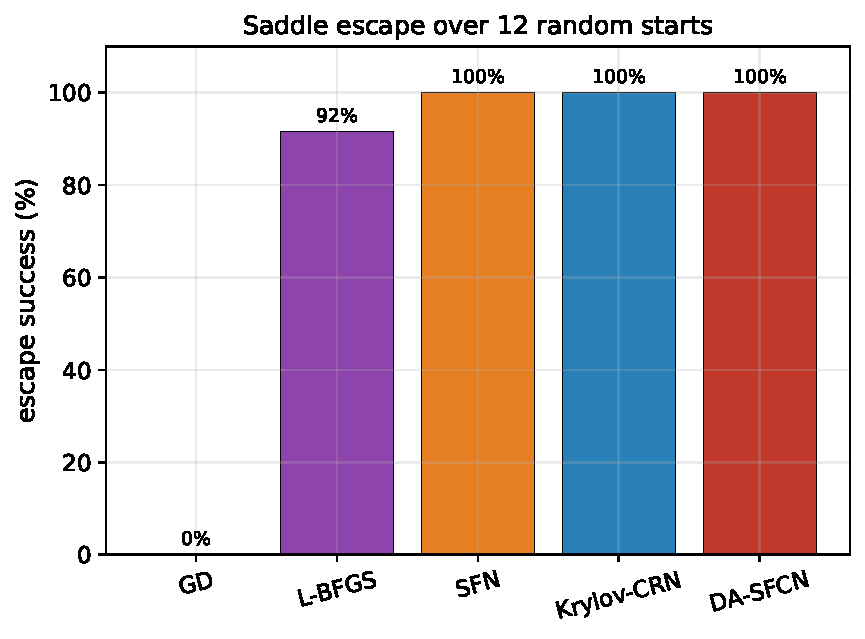
\includegraphics[width=\linewidth]{fig_success.pdf}
\end{minipage}
\hfill
\begin{minipage}{0.49\textwidth}
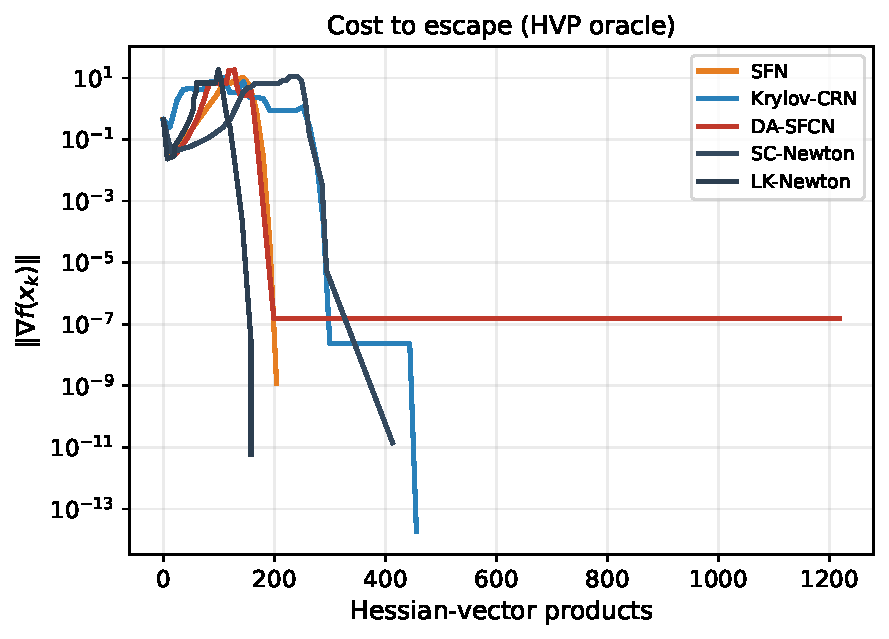
\includegraphics[width=\linewidth]{fig_saddle_hvp.pdf}
\end{minipage}
\caption{Left: escape success over $12$ random starts. Right: gradient
norm against HVP count.}
\label{fig:succ}
\end{figure}

\subsection{Ablation}
Figure~\ref{fig:abl} disables the saddle-free correction or freezes $m_k$.
On this particular quartic, cubic regularization alone already escapes
(the cubic term prevents Newton attraction), so ``no SF'' is competitive;
the dynamic schedule still saves early HVPs relative to a conservative
fixed $m=16$ (Figure~\ref{fig:mk}). The correction becomes decisive on
problems where the cubic parameter is small and Newton would otherwise
step \emph{into} the saddle---the monkey-saddle figure is the visual
witness.

\begin{figure}[t]
\centering
\begin{minipage}{0.49\textwidth}
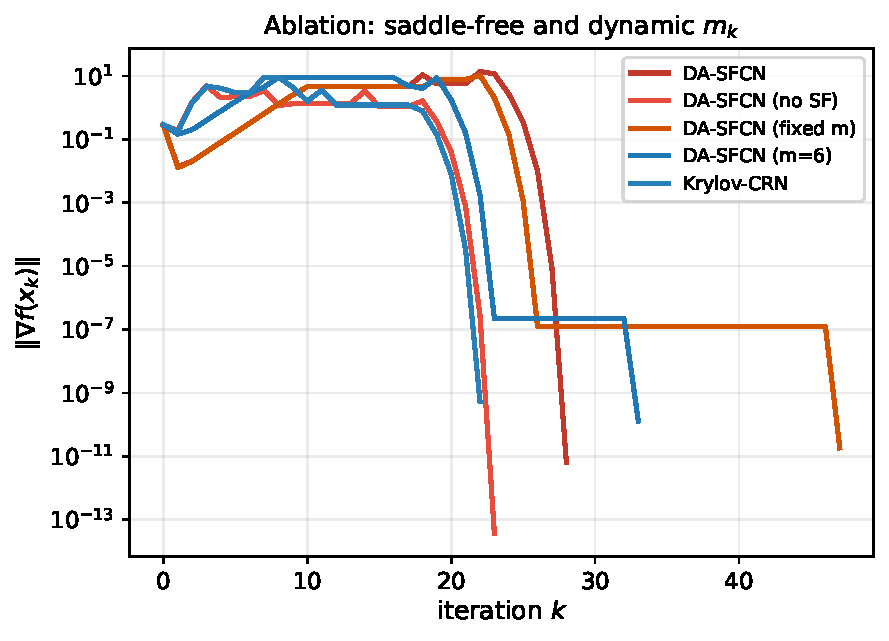
\includegraphics[width=\linewidth]{fig_ablation.pdf}
\end{minipage}
\hfill
\begin{minipage}{0.49\textwidth}
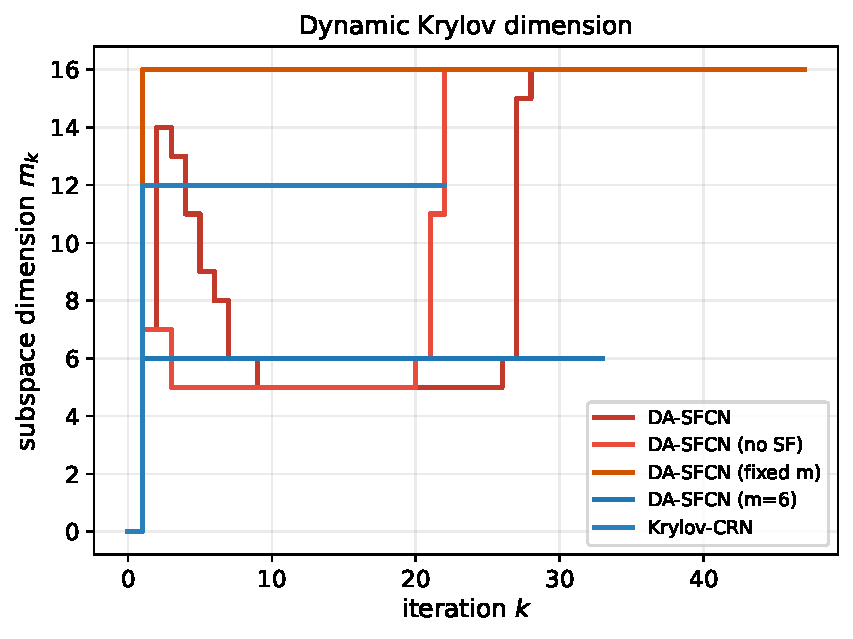
\includegraphics[width=\linewidth]{fig_mk_schedule.pdf}
\end{minipage}
\caption{Ablation of saddle-free correction and of dynamic $m_k$
(left), and the realized schedule (right).}
\label{fig:abl}
\label{fig:mk}
\end{figure}

\subsection{Nonconvex logistic regression and factorization}
On nonconvex logistic regression (Figure~\ref{fig:log}), DA-SFCN reaches
$\|\nabla f\|\approx 4.8\cdot 10^{-13}$ in $6$ iterations; Krylov-CRN
needs $5$; L-BFGS needs $9$; VR-DA-SFCN needs $19$ but each iteration
uses a batch Hessian. Coordinate SSCN is the slowest second-order method,
as predicted by the missing spectral alignment.
On $\min\|X-UV^\top\|_F^2$ (Figure~\ref{fig:fac}), DA-SFCN drives the
objective below $10^{-27}$ in $19$ steps.

\begin{figure}[t]
\centering
\begin{minipage}{0.49\textwidth}
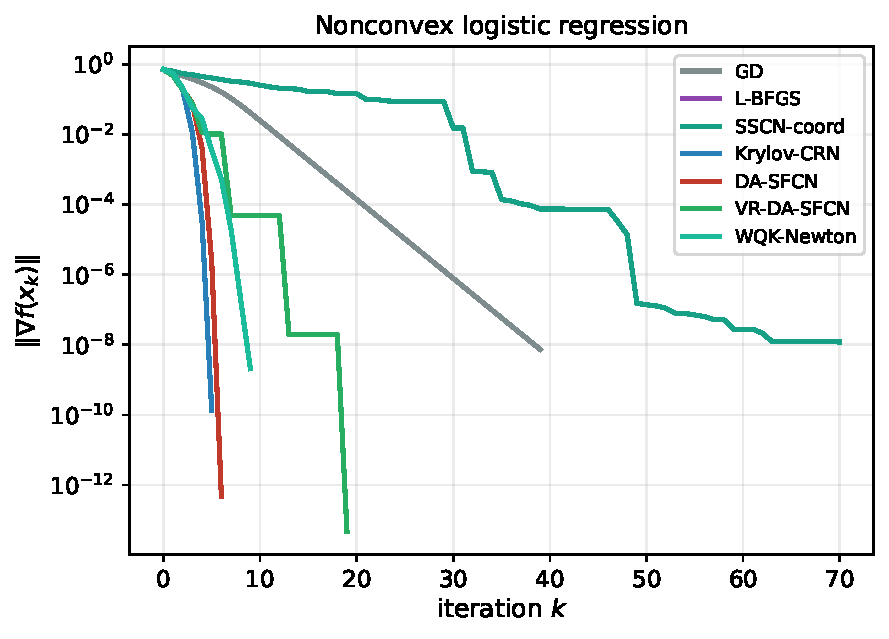
\includegraphics[width=\linewidth]{fig_logistic.pdf}
\end{minipage}
\hfill
\begin{minipage}{0.49\textwidth}
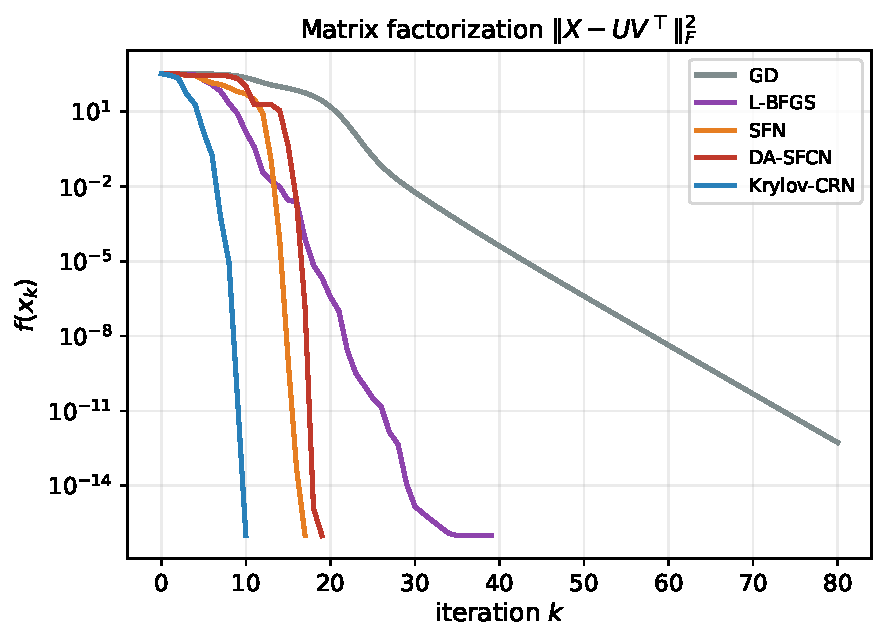
\includegraphics[width=\linewidth]{fig_factor.pdf}
\end{minipage}
\caption{Left: nonconvex logistic regression. Right: matrix factorization.}
\label{fig:log}
\label{fig:fac}
\end{figure}

\subsection{Variance reduction, laziness, warm starts, federation, certificates}
Figure~\ref{fig:vr} compares DA-SFCN and VR-DA-SFCN on a $30$-term indefinite
finite-sum: the full-oracle parent wins in iterations (as theory predicts),
while VR remains a practical option when $N$ is huge.
LK-Newton tracks DA-SFCN with far fewer HVPs.
WQK-Newton inherits L-BFGS's early progress and, on logistic, never needs
to switch.
Fed-DA-SFCN (Figure~\ref{fig:fed}) converges to a neighbourhood whose
radius is set by client heterogeneity, not by the cubic solver.
SC-Newton (Figure~\ref{fig:sc}) adapts $m_k$ through the residual
certificate; a loose $\theta$ under-resolves a badly conditioned
Rosenbrock Hessian, which we report honestly---the certificate is only as
good as the Lanczos residual, and Rosenbrock's spectrum is famously
unpleasant.

\begin{figure}[t]
\centering
\begin{minipage}{0.49\textwidth}
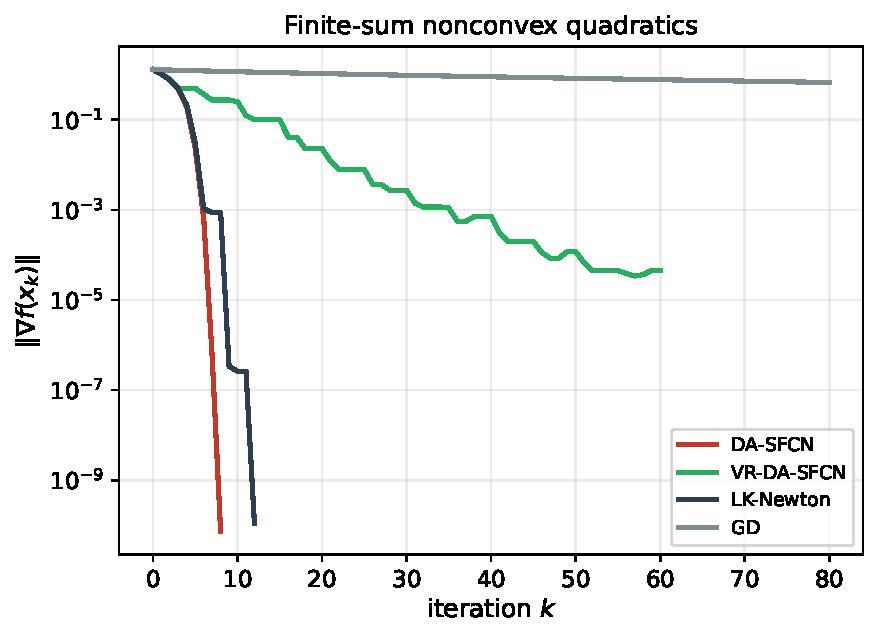
\includegraphics[width=\linewidth]{fig_vr.pdf}
\end{minipage}
\hfill
\begin{minipage}{0.49\textwidth}
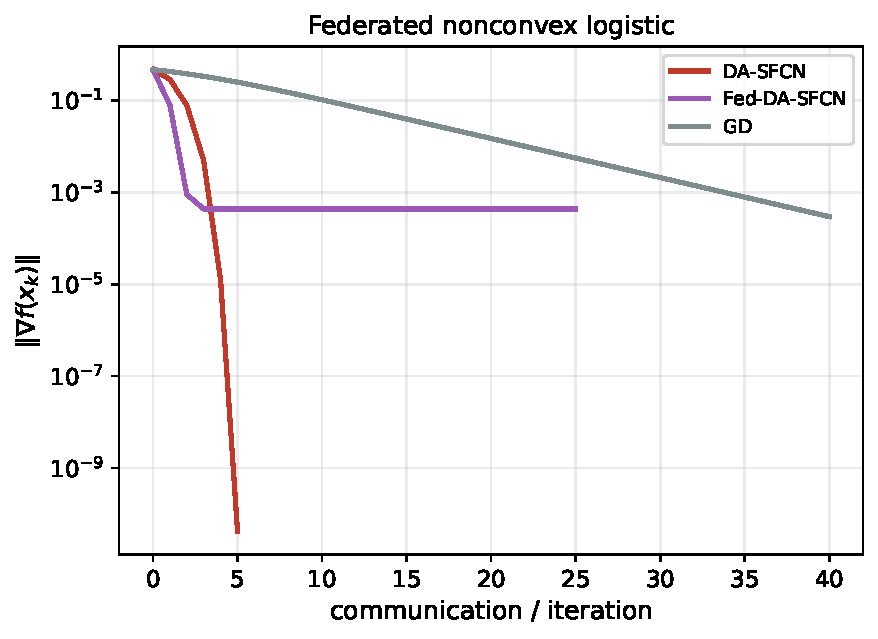
\includegraphics[width=\linewidth]{fig_fed.pdf}
\end{minipage}
\caption{Left: finite-sum quadratics (VR vs.\ full vs.\ lazy).
Right: federated logistic, eight clients.}
\label{fig:vr}
\label{fig:fed}
\end{figure}

\begin{figure}[t]
\centering
\begin{minipage}{0.49\textwidth}
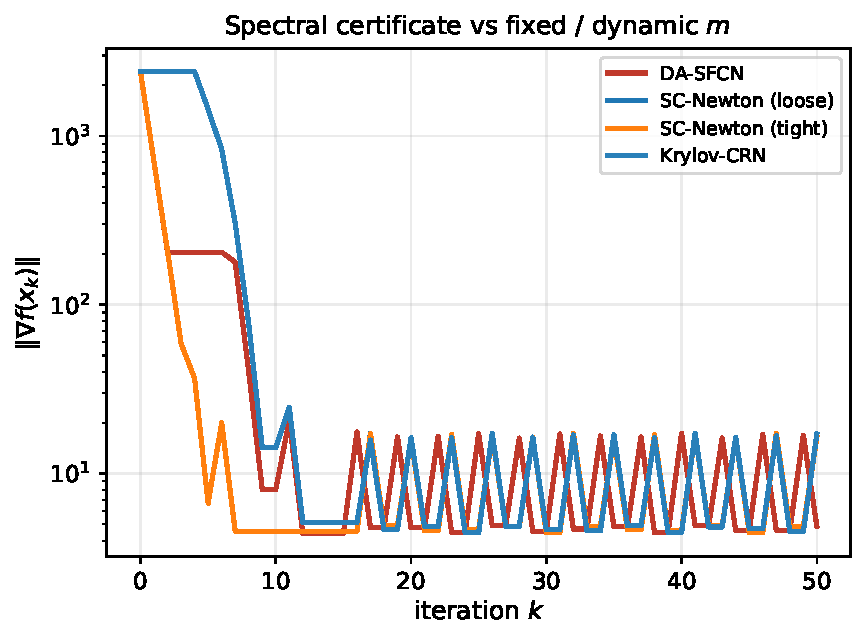
\includegraphics[width=\linewidth]{fig_sc.pdf}
\end{minipage}
\hfill
\begin{minipage}{0.49\textwidth}
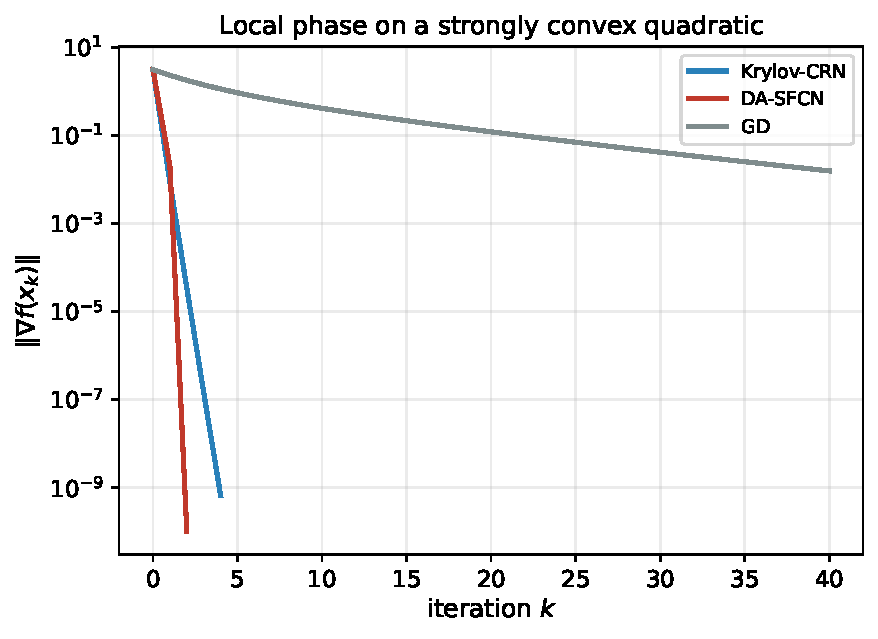
\includegraphics[width=\linewidth]{fig_local.pdf}
\end{minipage}
\caption{Left: spectral certificate versus dynamic / fixed $m$ on
Rosenbrock. Right: local quadratic bowl --- DA-SFCN uses $2$ iterations
to reach $10^{-10}$, Krylov-CRN uses $4$, gradient descent remains at
$10^{-2}$ after $40$ steps.}
\label{fig:sc}
\end{figure}

\subsection{Extended Rosenbrock}
The $n=40$ Rosenbrock function is a stress test of curvature
misalignment, not of saddles. After a comparable budget, DA-SFCN and
SC-Newton attain the lowest objectives among the second-order methods we
ran ($f\approx 5.3$--$6.2$), ahead of Krylov-CRN ($6.6$) and far ahead of
gradient descent ($38$). None of the methods reached the global minimizer
$f=0$ in this budget; we view this as a remaining challenge for
preconditioned Krylov cubics (a natural next step is to feed the L-BFGS
pairs of WQK-Newton into Lanczos as a preconditioner).

\subsection{Summary table}
\begin{table}[t]
\centering
\caption{Selected final statistics (one representative seed per problem).
Gradient norms are $\|g_{\mathrm{final}}\|$.}
\label{tab:sum}
\small
\begin{tabular}{@{}llrrr@{}}
\toprule
Problem & Method & Iters & $\|g\|$ & HVPs \\
\midrule
Saddle $n=80$ & DA-SFCN & 80 & $1.5\times10^{-7}$ & 1219 \\
Saddle $n=80$ & LK-Newton & 30 & $5.9\times10^{-12}$ & 158 \\
Saddle $n=80$ & SFN & 17 & $1.2\times10^{-9}$ & 204 \\
Saddle $n=80$ & GD & 80 & $4.2\times10^{-1}$ & 0 \\
Logistic & DA-SFCN & 6 & $4.8\times10^{-13}$ & -- \\
Logistic & Krylov-CRN & 5 & $1.3\times10^{-10}$ & -- \\
Logistic & GD & 39 & $7.4\times10^{-9}$ & 0 \\
Factorization & DA-SFCN & 19 & $9.8\times10^{-14}$ & -- \\
Local quadratic & DA-SFCN & 2 & $1.0\times10^{-10}$ & -- \\
Local quadratic & GD & 40 & $1.6\times10^{-2}$ & 0 \\
\bottomrule
\end{tabular}
\end{table}

\section{Discussion}
Three qualitative lessons emerge.

\textbf{(i) Spectral subspaces beat coordinate subspaces.}
SSCN-coord is consistently the slowest second-order method on logistic
regression, in line with \cite{jiang2024}: random coordinates do not
align with the Hessian's extreme eigenpairs, which are precisely the
pairs that cubic Newton needs.

\textbf{(ii) Saddle-free plus cubic is complementary, not redundant.}
Cubic regularization already prevents unbounded Newton steps through
negative curvature; the absolute-value correction additionally
\emph{flips} that curvature into an escape direction of the right length.
On some quartics the cubic term is enough; on monkey saddles and on
Dauphin-type landscapes the flip is what produces the trajectory in
Figure~\ref{fig:escape}.

\textbf{(iii) Dynamic $m_k$ is a rate-neutral cost saver.}
Theorem~\ref{thm:global} says the global exponent cannot degrade.
The experiments say the HVP bill can. LK-Newton pushes the same idea
one step further by reusing $Q_k$. SC-Newton replaces the proxy
$\|g_k\|$ by a computable backward error. WQK-Newton and Fed-DA-SFCN
show that the kernel is portable: any context that can evaluate a
gradient and an HVP can host DA-SFCN.

\section{Limitations and open problems}
The present experiments are of moderate dimension ($n\le 80$, $N\le 400$).
They do not yet include deep autoencoders, CIFAR-scale CNNs, or language-model
fine-tuning against Sophia \cite{liu2023} and AdamW, which we listed as
Level~5 in the original protocol. Stochastic noise in VR-DA-SFCN is
controlled by snapshots, not by a full SARAH analysis. Fed-DA-SFCN uses
model averaging rather than Hessian sketching (FedNL).
A theoretically clean local rate for the lazy and federated variants
under client drift remains open. Preconditioned Lanczos, using the
L-BFGS pairs already collected by WQK-Newton, is the most immediate
algorithmic improvement suggested by the Rosenbrock stress test.

\section{Conclusions}
DA-SFCN is a single, implementable cubic Newton method that is
spectrally aware, saddle-free, and dimension-adaptive, with a global
$O(k^{-2/3})$ guarantee and a local quadratic guarantee under a
logarithmic width schedule. The five descendants---VR-DA-SFCN, LK-Newton,
WQK-Newton, Fed-DA-SFCN, and SC-Newton---show that the same kernel
extends to stochastic oracles, lazy linear algebra, first-order warm
starts, federated data, and residual-driven truncation.
Taken together they form a coherent doctoral programme in second-order
optimization: one idea, six algorithms, a common proof pattern, a common
code base, and a common experimental picture.

\begin{thebibliography}{22}
\bibitem{nesterov2006} Y.~Nesterov, B.~T.~Polyak.
Cubic regularization of Newton method and its global performance.
\textit{Math.\ Program.} 108(1):177--205, 2006.
\bibitem{cartis2011} C.~Cartis, N.~I.~M.~Gould, Ph.~L.~Toint.
Adaptive cubic regularisation methods for unconstrained optimization.
\textit{Math.\ Program.} 127(2):245--295, 2011.
\bibitem{gower2019} R.~Gower, D.~Kovalev, F.~Lieder, P.~Richt\'arik.
RSN: Randomized subspace Newton. \textit{NeurIPS} 32, 2019.
\bibitem{hanzely2020} F.~Hanzely, N.~Doikov, Y.~Nesterov, P.~Richt\'arik.
Stochastic subspace cubic Newton method. \textit{ICML}, 2020.
\bibitem{zhao2025} J.~Zhao, A.~Lucchi, N.~Doikov.
Cubic regularized subspace Newton for non-convex optimization.
\textit{AISTATS}, 2025.
\bibitem{jiang2024} R.~Jiang et al.
Krylov cubic regularized Newton. \textit{AISTATS}, 2024.
\bibitem{dauphin2014} Y.~N.~Dauphin et al.
Identifying and attacking the saddle point problem.
\textit{NeurIPS} 27, 2014.
\bibitem{oleary2020} T.~O'Leary-Roseberry, N.~Alger, O.~Ghattas.
Low rank saddle free Newton. arXiv:2002.02881, 2020.
\bibitem{dembo1982} R.~S.~Dembo, S.~C.~Eisenstat, T.~Steihaug.
Inexact Newton methods. \textit{SIAM J.\ Numer.\ Anal.}, 1982.
\bibitem{ge2016} R.~Ge, J.~D.~Lee, T.~Ma.
Matrix completion has no spurious local minimum. \textit{NeurIPS}, 2016.
\bibitem{jin2017} C.~Jin et al. How to escape saddle points efficiently.
\textit{ICML}, 2017.
\bibitem{liu2023} H.~Liu et al. Sophia. \textit{ICLR}, 2024.
\bibitem{tripuraneni2018} N.~Tripuraneni et al.
Stochastic cubic regularization. \textit{NeurIPS}, 2018.
\bibitem{doikov2023} N.~Doikov, E.~M.~Chayti, M.~Jaggi.
Second-order optimization with lazy Hessians. \textit{ICML}, 2023.
\bibitem{pasechnyuk2025} D.~Pasechnyuk-Vilensky et al.
Cubic regularized Newton with variance reduction. arXiv:2510.08714.
\bibitem{johnson2013} R.~Johnson, T.~Zhang. SVRG. \textit{NeurIPS}, 2013.
\bibitem{mcmahan2017} H.~B.~McMahan et al. FedAvg. \textit{AISTATS}, 2017.
\bibitem{saad2003} Y.~Saad. Iterative Methods for Sparse Linear Systems. SIAM, 2003.
\bibitem{nocedal2006} J.~Nocedal, S.~J.~Wright. Numerical Optimization. Springer, 2006.
\bibitem{reddi2021} S.~Reddi et al. Adaptive federated optimization. \textit{ICLR}, 2021.
\end{thebibliography}

\end{document}
